\chapter{EUPHONY: unification of malware labels}
\label{chapter:euphony}

\begin{quote}
{\itshape
Android malware is now pervasive and evolving rapidly. Thousands of malware samples are discovered every day with new models of attacks. The growth of these threats has come hand in hand with the proliferation of collective repositories sharing the latest specimens. Having access to a large number of samples opens new research directions aiming at efficiently vetting apps. However, automatically inferring a reference dataset from those repositories is not straightforward and can inadvertently lead to unforeseen misconceptions. On the one hand, samples are often mislabeled as different parties use distinct naming schemes for the same sample. On the other hand, samples are frequently misclassified due to conceptual errors made during labeling processes.
    
In this chapter, we mine antivirus labels and analyze the associations between all labels given by different vendors to systematically unify common samples into family groups. The key novelty of our approach, named EUPHONY, is that no apriori knowledge on malware families is needed. We evaluate EUPHONY using reference datasets and more than 400 thousand additional samples outside of these datasets. Results show that EUPHONY can accurately label malware with a fine-grained clustering of families while providing competitive performance against the state-of-the-art.

\vfill

\begin{center}
Euphony: Harmonious Unification of Cacophonous \\ Anti-Virus Vendor Labels for Android Malware

Médéric Hurier, Guillermo Suarez-Tangil, Santanu Kumar Dash, \\ Tegawendé F. Bissyande, Yves le Traon, Jacques Klein, Lorenzo Cavallaro

The 14th International Conference on Mining Software Repositories (MSR) \\
May 20-21, 2017. Buenos Aires, Argentina

Source code: \url{https://github.com/fmind/euphony}

Dataset: \url{https://androzoo.uni.lu/labels}
\end{center}
}
\end{quote}


\localtableofcontents{}

Machine learning based approaches rely on ground truth datasets to training and evaluate statistical models.
Unfortunately, as Rossow et al.~\cite{rossow_prudent_2012} pointed out, the literature exhibits several shortcomings, including a lack of correctness, transparency, and realism in the handling of malware datasets.
In particular, reliable malware labels are a necessary input to guarantee the quality of both malware detection and classification models.

Malware labeling, however, is not a trivial task.
Manual labeling, where a human analyst inspects the actions of the malware in a bid to classify them, is prohibitively expensive, given the number of malware samples discovered every day.
In such a setting, it is reasonable to rely on the collective judgment of antivirus vendors who specialize in malware labeling.
However, deriving a unified label from labels attached to samples by antivirus vendors is difficult.
Inconsistencies in antivirus labels are indeed typical.
As we reviewed in the previous chapter, several inconsistencies were found in malware labels such as a global lack of consensus and a high degree of divergence.
These inconsistencies are due to both naming disagreements~\cite{kantchelian_better_2015} across vendors, and also a lack of adopted standards\footnote{CARO and CME conventions are not widely used by antivirus vendors.} for naming malware.

Previous works have relied on simple heuristics to come up with unified labels based on assessment reports of antivirus vendors.
For the case of labeling malware as benign or malicious, techniques have labeled a sample as malicious if at least one antivirus vendor flags it as malicious or at least the majority of antivirus vendors have flagged it as malicious~\cite{arp_drebin:_2014, lindorfer_marvin:_2015}.

While such heuristics work for flagging samples as malicious or benign, labeling samples with the specific class they belong to is fraught with difficulties.
Antivirus vendors can choose different norms to name classes, prefixing qualifying attributes such as attack type (e.g., \emph{Trojan}) or platform (e.g., \emph{Android}) to the label.
What further complicates things is that it is not uncommon for typographic and orthographic inconsistencies to creep into the labeling process not just across vendors but sometimes even for the same vendor.
Consequently, a sample's full antivirus label is a poor indicator of its generic family name.
For example, the family name $Adrd$ is ``lost'' in the full antivirus label \textit{Android.Trojan.Adrd.A (B)}.

In this work, we present EUPHONY, a tunable antivirus labeling system that can systematically extract information from antivirus labels and learns their patterns and vocabulary over time.
EUPHONY is an inference based system, which allows for end to end automation, relieving practitioners from the need to collect, aggregate and verify malware families manually.
EUPHONY label unification scheme is also vendor agnostic.
No specific rules about antivirus engines (e.g., which label parts are suffixes to be removed) are encoded in the process as these rules are inferred from the available antivirus labels data.

Figure~\ref{figure:euphony:architecture} illustrates the high-level overview of the architecture of EUPHONY.
As input, the tool takes a collection of antivirus scanning reports.
Such reports can be readily obtained from online services such as {\em VirusTotal}~\cite{noauthor_virustotal_nodate}, which gathers shared intelligence from several antivirus engines.
Then for each sample, EUPHONY performs the following tasks:

\begin{figure}[!ht]
	\centering
	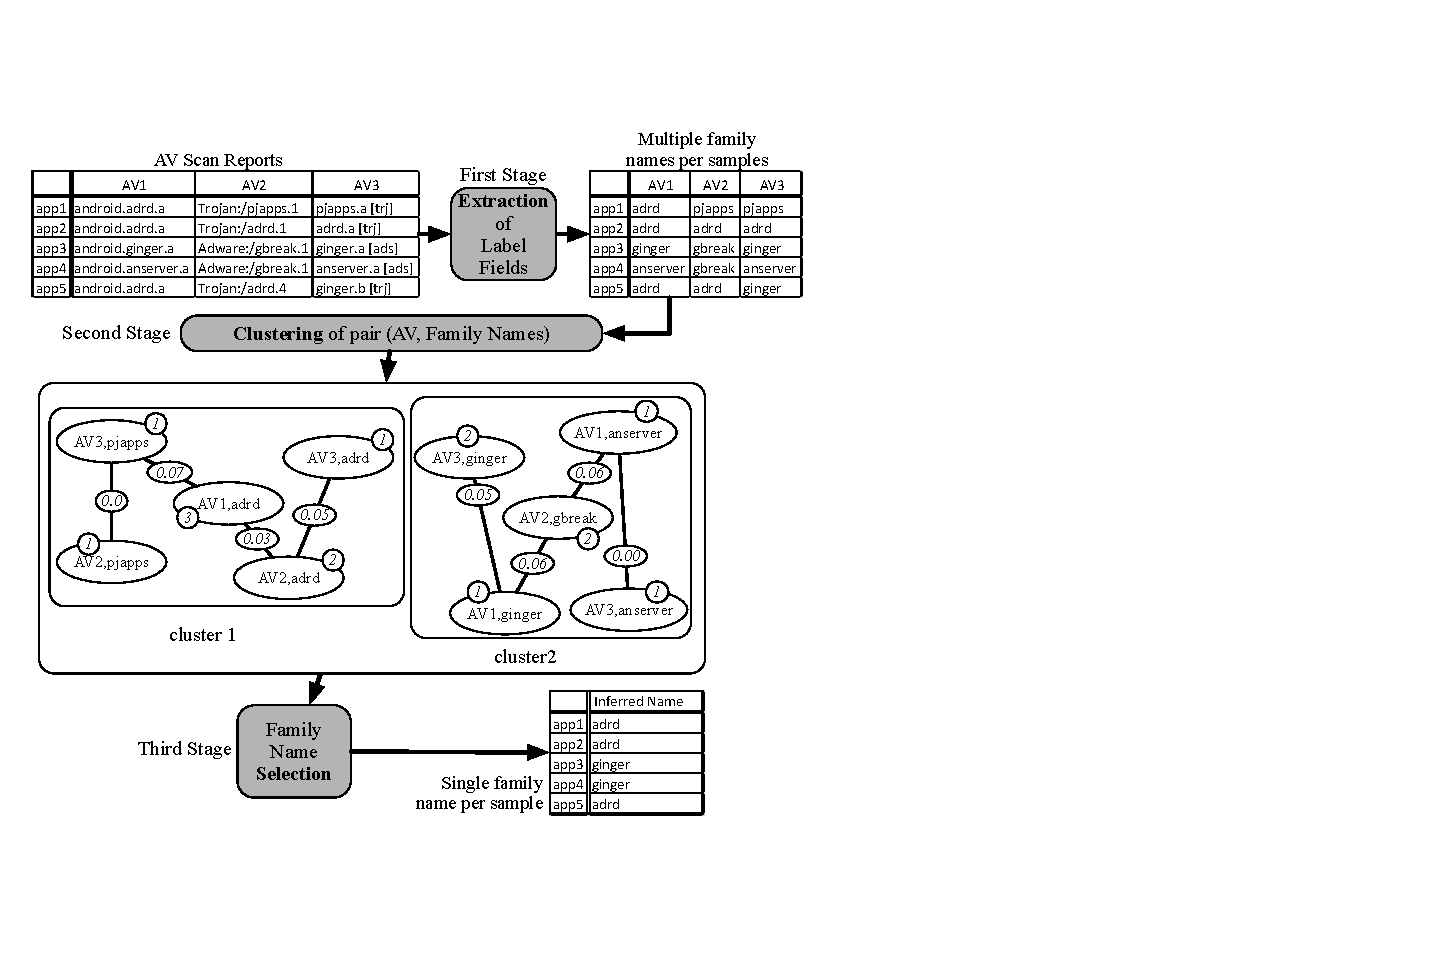
\includegraphics[width=\linewidth]{figures/euphony/architecture04.pdf}
	\caption{Overview of EUPHONY architecture}
	\label{figure:euphony:architecture}
\end{figure}

\begin{itemize}
	\item \textbf{First stage:} antivirus labels are pre-processed to derive the family name assigned by each vendor to a given sample. This task allows EUPHONY to deal with different unstructured naming patterns used by the antivirus and the lack of convention motivates it.

	\item \textbf{Second stage:} This task aims at structuring the relationship between different family names and provides the most appropriate associations between them. EUPHONY analyses both the correlation and the overlap between all family names to understand (i) {\em mislabeled} and (ii) {\em misclassified} samples. While mislabeling a sample generally happens when many antiviruses use a different naming scheme for the same family (e.g.: $DroidKungFu$ vs. $DrdKngFu$), misclassifying a sample is usually associated with a conceptual error made by an antivirus---with respect to the others (e.g., a vendor labels a sample as $GingerMaster$ while the others decide that belongs to $DroidKungFu$).

	\item \textbf{Third stage:} This task aims at bringing consensus between the different vendors and outputs the most appropriate family name for a given sample. Although our framework can also output a set of family names for a sample (i.e., synonyms), for the sake of simplicity, we only report the most prevalent one.
\end{itemize}

We next describe the details of each of the components in EUPHONY as well as the choices made during their design and implementation.
\section{Definition of labeling process}
\subsection{Antivirus labels}

\begin{definition}[Antivirus label]
	An antivirus label $l$ is a sequence of words (i.e., alphanumerical tokens) $w_i$ divided by separators (i.e., blanks and punctuation signs) $u_j$. Formally, $l = (w_1, u_1, \dots, u_n, w_{n+1})$.
\end{definition}

\texttt{Android.Trojan.Adrd.A (B)} is a concrete example of such a label, where `.' ($dot$), `$($', `$)$' ($parentheses$), and `\textvisiblespace' ($space$) are the separators and $Android$, $Trojan$, $Adrd$, $A$, and $B$ are the words.

\begin{definition}[Antivirus label field]
	A label field $f$ represents the category of a given word $w_i$.
\end{definition}

\noindent
The word $Android$ in \texttt{Android.Trojan.Adrd.A~(B)} indicates the target platform of the malware, while $Trojan$ and $Adrd$ indicate its type and family respectively.
Overall, we define 4 fields that match details required in the CARO naming convention~\cite{skulason_caro_nodate}: \textbf{type} (the kind of threat, i.e., trojan, worm, etc.), \textbf{platform} (the OS that the threat is designed to work on, i.e., Windows, Android, etc.), \textbf{family} (the group of threats it is associated with in terms of behavior), \textbf{information} (extra description of this threat, including its variant).

Grammars described in Table~\ref{table:euphony:lexing} and Table~\ref{table:euphony:parsing} below provide the lexing rules used by EUPHONY to tokenize antivirus labels.

\begin{table}[!ht]
\centering
    \caption{Lexing rules of EUPHONY}
    \resizebox{0.5\linewidth}{!}{
        \begin{tabular}{lcl}
            \textit{<family>} &::=& [:alpha:]\{3,\} \\
            \textit{<type>} &::=& [:alpha:]\{2,\} \\
            \textit{<info>}&::=& [:alnum:]+ \\
            \textit{<plat>} &::=& [:alnum:]\{2,\} \\
            \textit{<sep>} &::=& ([:punct:] | [:blank:])+
        \end{tabular}
    }
    \label{table:euphony:lexing}
\end{table}


\begin{table}[!ht]
    \centering
    \caption{Parsing rules of EUPHONY}
    \resizebox{0.6\linewidth}{!}{
        \begin{tabular}{lcl}
        \textit{<word>} &::=& <family> | <type> | <plat> | <info> \\
        \textit{<label>} &::=& <word> | <sep> | <label> \\
        \end{tabular}
    }
    \label{table:euphony:parsing}
\end{table}


\begin{definition}[Antivirus labeling pattern]
	Given an antivirus \emph{av}, its corresponding antivirus labeling Pattern, noted $p_{av}$ represents the syntax of its labels, i.e., how the different fields are combined to form its labels.
\end{definition}

We provide in Table~\ref{table:euphony:fields} some illustrative examples of antivirus labels, their fields, and their associated labeling patterns.

\begin{table}[!ht]
    \centering
    \caption{Examples of antivirus labeling patterns}
    \resizebox{0.85\linewidth}{!}{
        \begin{tabular}{|c|c|cccc|}
            \hline
            \textbf{Label}               & \textbf{AV Pattern}                       & \textbf{Family} & \textbf{Type} & \textbf{Plat.} & \textbf{Info} \\
            \hline
            Android.Trojan.Adrd & <plat>.<type>.<name> & adrd         & trojan     & android        & --           \\
            \hline
            Trojan:/Adrd.b  &	<type>:/<name>.<info>       & adrd         & trojan     & --      & b            \\
            \hline
            Android:PjApps [Trj]    & <plat>:<name> [<type>]      & pjapps       & trj        & android        & --           \\
            \hline
            Troj.PjApps (kcloud)    & <type>.<name> (<info>)          & pjapps       & troj       & --             & kcloud      \\
            \hline
            Android/Adrd.5e2f & <plat>/<name>.<info>        & adrd         & --    & android        & 5e2f        \\
            \bottomrule
        \end{tabular}
    }
    \label{table:euphony:fields}
\end{table}

\subsection{Sample sets}
We define a labeling function $label\_of$ which associates a label to a pair $(av, app)$ of antivirus and application from a dataset:

\begin{definition}[Labeling function]
	Let $APP$ be a set of applications, $antivirus$ a set of antivirus, and $\mathcal{L}$ the set of associated labels.

	The function $label\_of:AV \times APP \rightarrow \mathcal{L}$ maps a pair of antivirus and application to a label.
\end{definition}

From a given label, we further define a family function $family\_of$ which extracts the family field value.

\begin{definition}[Family function]
	Let $AV$ be a set of antivirus, $APP$ a set of applications. Let be $\mathcal{L}$ the set of labels such as $\mathcal{L}= label\_of(AV,APP)$,
	and $\mathcal{F}$ a set of associated family names.

	The function $family\_of:AV \times \mathcal{L} \rightarrow \mathcal{F}$ maps a pair of antivirus and label to a family name.
\end{definition}

For a given $AV$, we put together apps with the same family name in a set that we call \emph{Sample Set}.
More formally:

\begin{definition}[Sample set]
	Let $APP=(app_1, app_2,... , app_n)$ be a set of app samples, and $\mathcal{F}=(f_1, f_2, ..., f_k)$ a set of associated families.
	For a given antivirus \emph{av}, the sample set $S_{av,f_j}$ defines the set of apps with the same family name $f_j$.
	More formally,
	\[
		\forall j \in (1,...,k), S_{av,f_j} = \{app_x \in APP | family\_of(av,app_x) = f_j\}
	\]
\end{definition}

\subsection{Metrics}
Sample sets can be disjoint or overlapping, and may be imbalanced.
For instance, the sample sets represented in the left of Figure~\ref{figure:euphony:samples} are imbalanced as the number of samples associated with the family name $f_i$ by $av_a$ is much smaller than the number of samples associated with family name $f_j$ by $av_b$.
Understanding when a sample set is imbalanced is important when weighting the relevance of a label over another in a dataset.

\begin{figure}[!ht]
        \centering
	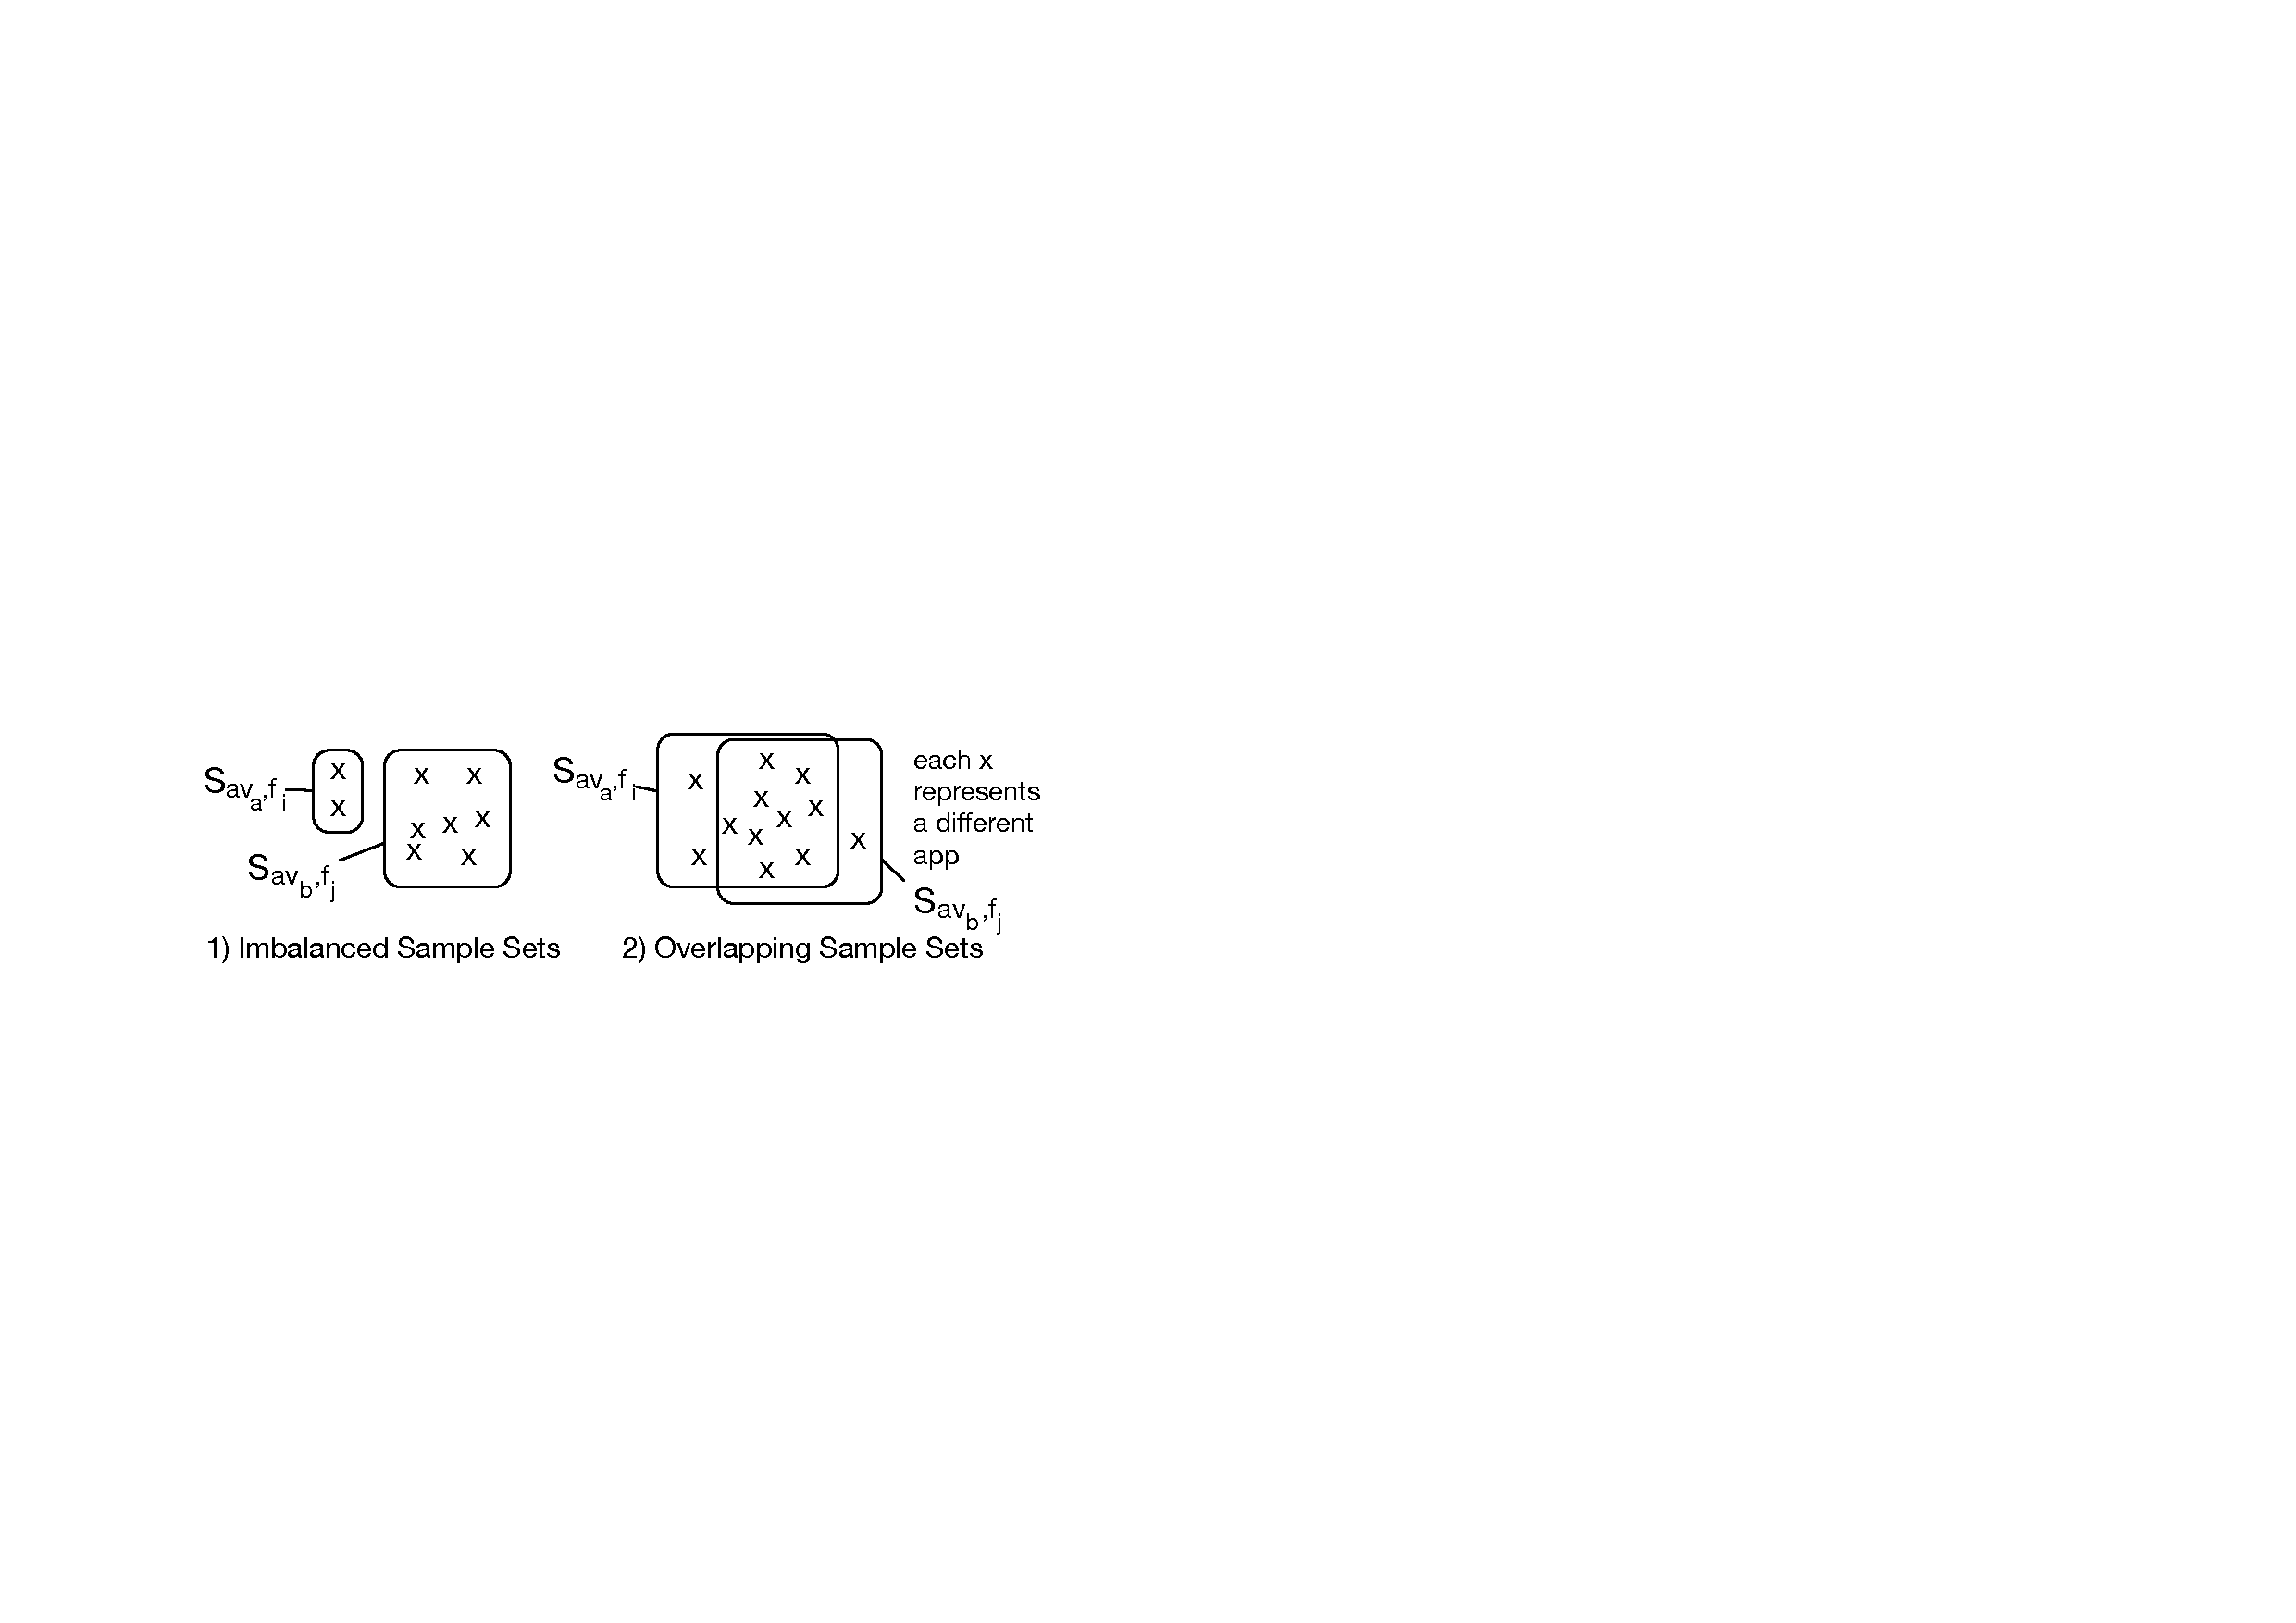
\includegraphics[width=0.8\linewidth]{figures/euphony/samples.pdf}
	\caption{Examples of application sample sets}
	\label{figure:euphony:samples}
\end{figure}

\begin{definition}[Imbalance metric]
	Given two sample sets $S_{av_a,f_i}$ and $S_{av_b,f_j}$, we define the \emph{Imbalance} metric as the complement between the minimum and maximum cardinality of the two sample sets, formalized in Equation~\ref{equation:imbalance}.
	\begin{equation}
		Im(S_{av_a,f_i}, S_{av_b,f_j}) = 1 - \frac{\min(|S_{av_a,f_i}|, |S_{av_b,f_j}|)}{\max(|S_{av_a,f_i}|, |S_{av_b,f_j}|)}
		\label{equation:imbalance}
	\end{equation}
\end{definition}

When both sets $S_{av_a,f_i}$ and $S_{av_b,f_j}$ have the same cardinality, there is no imbalance, and $Im$ is equal to $0$.
In contrast, imbalance $Im$ gets close to 1 as $S_{av_a,f_i}$ contains fewer apps and $S_{av_b,f_j}$ contains a lot more.

The right part of Figure~\ref{figure:euphony:samples} depicts overlapping sample sets, i.e., a scenario where several apps have been associated at the same time with $f_i$ and $f_j$ by $av_a$ and $av_b$ respectively.
This setting suggests that, despite syntactic differences between both family names $f_i$ and $f_j$, the family names may characterize the same information (e.g., they point to the same malware).
The notion of overlapping is essential to assess whether family names should be merged.
Thus, we define the exclusion metric which quantifies the degree of overlapping, or lack thereof.

\begin{definition}[Exclusion metric]
	Given two sample sets $S_{av_a,f_i}$ and $S_{av_b,f_j}$, we define the \emph{Exclusion Metric} as the complement of the ratio between the intersection cardinality of two sample sets $S_{av_a,f_i}$ and $S_{av_b,f_j}$ the cardinality of the smallest sample set.
	This metric is formalized by Equation~\ref{equation:exclusion}.
	\begin{equation}
		Ex(S_{av_a,f_i}, S_{av_b,f_j}) = 1 - \frac{|(S_{av_a,f_i} \cap S_{av_b,f_j})|}{\min(|S_{av_a,f_i}|, |S_{av_b,f_j}|)}
		\label{equation:exclusion}
	\end{equation}
\end{definition}

When the sets $S_{av_a,f_i}$ and $S_{av_b,f_j}$ share no app, there is no overlapping as their intersection is empty, and {\em Ex} is at its maximum at $1$.
In contrast, as the overlapping gets higher, {\em Ex} gets close to $0$.

Given that family names may contain small syntactic differences, we consider a distance function to relax the equality constraint on strings.
To that end, we define our String distance based on the Sørensen–Dice index~\cite{dice_measures_1945}.

\begin{definition}[Distance metric of family names]
	The distance metric of family names is computed as the string distance between two family names $f_i$ and $f_j$:
	\begin{equation}
		D(f_i, f_j) = 1 - dice(f_i, f_j)
	\end{equation}
\end{definition}

Finally, we measure how two family names $f_i$ and $f_j$, given by the antivirus $av_a$ and $av_b$ respectively, are far to designate the same malware family.
More specifically, we compute the distance between two samples sets $S_{av_a,f_i}$ and $S_{av_b,f_j}$ by combining the imbalance, exclusion as well as the string distance metrics that we introduced.
The following equation provides the formula that we use:

\begin{definition}[Sample set distance metric]
	Given two sample sets $S_{av_a,f_i}$ and $S_{av_b,f_j}$, we define the \emph{Sample Set Distance Metric} as follows:

	\begin{multline}
		W(S_{av_a,f_i}, S_{av_b,f_j}) =\alpha \times Ex(S_{av_a,f_i}, S_{av_b,f_j}) + \beta \times Im(S_{av_a,f_i}, S_{av_b,f_j}) + \gamma \label{eq:weight} \times D(f_i, f_j)
	\end{multline}
\end{definition}

Where $\alpha$, $\beta$ and $\gamma$ are weight coefficients for adjusting the importance of the different metrics leveraged to compute the sample set distance.
First and foremost, we consider that two family names are close to each other only if there is a strong overlap (i.e., low exclusion) between their associated sample sets.
Thus, for example, it is not opportune to consider two family names as similar if they do not occur concurrently for the same samples.
Consequently, the value of $\alpha$ will reflect the importance of the {\em Ex} metric.
Second, the imbalance of sample sets is considered to account for the degree of granularity within malware families.
For example, an antivirus might assign two family names to a sample set (e.g., $ADRD$, $Pjapps$) while another antivirus might use only one (e.g., $Pjapps$) family name for all samples in the set.
Finally, the impact of typos, which may increase distances between sample sets, requires the string distance to be the least weighted.
We have empirically found that a difference of an order of magnitude captures the best relative importance among the coefficients.
Thus, in EUPHONY, we set $\alpha$, $\beta$ and $\gamma$ to $1$, $\frac{1}{10}$ and $\frac{1}{100}$ respectively.
\section{Extraction of label information}
An antivirus label is an informally structured string concatenating various pieces of information for describing the malware.
In the previous section, we have identified four recurrent fields in antivirus labels which are identifiable in labels: family, type, platform, and extra information.
Each vendor generally adopts a specific naming convention to represent and combine these fields in a string.
For example, while some vendors start with the platform first, followed by the type and the name; other vendors opt to put the type first or enclose it between square brackets at the end of the string.
We further note that antiviruses change their convention over time, varying field ordering and the punctuation signs that separate fields.
In this context, the normalization of their syntax cannot be achieved consistently via fixed rules such as regular expressions.

Another crucial constraint in parsing antivirus labels is the lack of a complete, universal and up-to-date lexicon.
Indeed, new types, platforms, and family names are continuously added by antivirus vendors to describe emergent threats, and refine the description of old threats.
Malware family names, in particular, are highly dynamic as new malicious behaviors appear regularly.

With these limitations in mind, we propose several heuristics for mapping antivirus label tokens to a lexical field.
The overall family name extraction process is described in Figure~\ref{figure:euphony:extraction}.
Given a collection of antivirus labels, the system can infer the most apparent fields and then iteratively move to the most challenging cases as its knowledge grows.
To bootstrap the process, EUPHONY builds on heuristics based rules, as well as a bare amount of vocabulary on some platform names (e.g., \textit{Android}) and types (e.g., \textit{trojan}).
The final output which is the family names given by each antivirus to the samples is obtained by inferring it from the sample's label for each vendor.

\begin{figure}
	\centering
	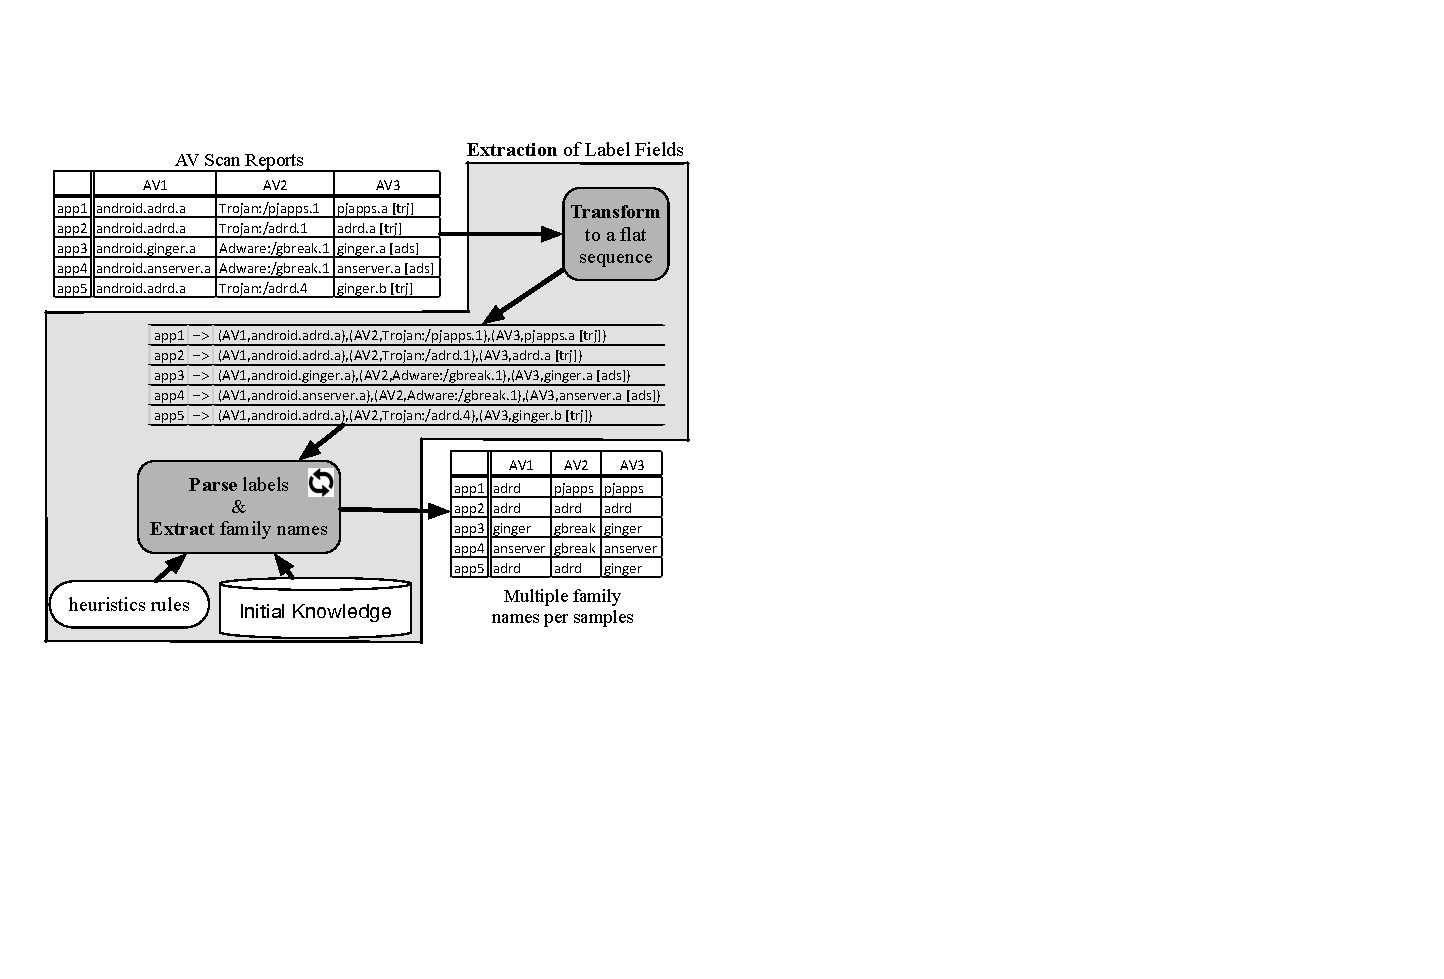
\includegraphics[width=\linewidth]{figures/euphony/extraction01.pdf}
	\caption{First stage - extraction of label fields from malware reports}
	\label{figure:euphony:extraction}
\end{figure}

\subsection{Parsing algorithm}
\begin{algorithm}[!ht]
    \caption{Incremental Parsing by EUPHONY}
    \begin{algorithmic}[1]
        \State{} $Mapping \gets [name, type, platform, information]$
        \Function{Parse}{$knowledge_{db}$, $heuristics$, $labels$}
        \State{} $mappings \gets \Call{map}{Mapping, labels}$
        \State{} $pqueue \gets \Call{prio-queue}{mappings}$
        \While{\Call{not-empty?}{$pqueue$}}
        \State{} $m \gets \Call{peek}{pqueue}$
        \For{$H$ in $heuristics$}
        \State{} $findings \gets \Call{h}{knowledge_{db}, m}$
        \State{} $\Call{merge}{m, findings}$
        \EndFor{}
        \If{\Call{complete?}{$m$}}
        \State{} \Call{Enrich}{$knowledge_{db}, m$}
        \Else{}
        \State{} \Call{Push}{$pqueue, m$}
        \EndIf{}
        \EndWhile{}
        \State{} \Return{} $mappings$
        \EndFunction{}
    \end{algorithmic}
    \label{algorithm:parse}
\end{algorithm}


The parsing algorithm is at the core of the labeling process and its steps are described in Algorithm~\ref{algorithm:parse}.
The process takes as input a set of labels, some defined heuristics and an initial knowledge database on malware lexicon.
First, the algorithm tokenizes each antivirus label and initializes the mappings between the tokens and the different label fields.
At this stage, a given token can be associated with all fields (name, type, platform or information).
To decide the unique field to which it should be assigned, the algorithm proceeds by iteratively eliminating improper assignment, starting with the easiest cases: the order of processing is conveyed by a priority queue (line 4), where mappings with the least amount of unknown fields are pushed at the head of the queue, while mappings with the most amount of unknown fields are pushed back at the end of the queue.
At each step, the algorithm takes the first mapping of the queue (line 6) and applies the heuristics based rules to collect more information about the mapping (line 8).
Then, it merges this information to create a new mapping.
In case of conflicts, the merge operation will always keep the oldest knowledge at its disposal.

If the mapping is complete at the end of this operation (line 11), i.e.,
if each token is associated with a single field, this mapping is removed from the queue and its information pieces are extracted to enrich the knowledge database (line 12).
Otherwise, the mapping is pushed back in the queue to be processed at a later iteration (line 14).
Once the queue is empty, the mapping list is returned with the complete list of associations (line 17).
To force early termination, EUPHONY provides a parameter for setting a maximum number of iterations performed by the algorithm.
\subsection{Heuristics rules}
We now provide details on the parameters of the algorithm.
In our current implementation, we rely on ten heuristic rules to find associations between words and fields.
These rules are listed in Table~\ref{table:euphony:heuristics}.

\begin{table}[!ht]
    \centering
    \resizebox{0.7\linewidth}{!}{
        \begin{tabular}{|p{0.5cm}|p{6cm}|p{3.75cm}|}
            \hline
            & \textbf{Property}                                                           &\textbf{Action}\\\hline
            1  & Word is associated to a known field in the database                         & associate the same field \\\hline
            2  & Word is suffixed by -ware                                                   & word is a type \\\hline
            3  & Word is between parenthesis                                                 & word is an info \\\hline
            4  & Word is between square brackets                                             & word is a type or info \\\hline
            5  & Only one family, type and platform per label                                & enforce when field is found \\\hline
            6  & Word is a synonym of a type or platform in the database (e.g.~troj, trojan) & associate the same field \\\hline
            7  & Word is the last token not associated to a field                            & word is a family \\\hline
            8  & Words are part of common word sentence                                      & words are info \\\hline
            9  & Label is compatible with a pattern of the same AV                           & associate fields based on pattern \\\hline
            10 & Given two remaining tokens, one is a common word and the other is not       & common word: information, other word: family \\
            \bottomrule
        \end{tabular}
    }
    \caption{Heuristics for mapping label words to fields}
    \label{table:euphony:heuristics}
\end{table}


Let us consider two of the rules to illustrate the associated action.
Rule 1 is the most straightforward heuristic.
During its execution, EUPHONY accesses the database to check if the word is already associated with a particular field.
In particular, the word {\em Android} is commonly known to match with the field \texttt{platform}.
Thus, Rule 1 can leverage existing knowledge to identify obvious fields.
Rule 9, on the other hand, is tuned to create more knowledge by inferring the field of an unknown token.
For example, given the antivirus label `ransom.android.pjapps' and its incomplete mapping [ransom: \texttt{?}, android: \texttt{platform}, pjapps: \texttt{family}], the algorithm can know at this stage that {\em ransom} is likely a \texttt{type}, and yield the following antivirus labeling pattern: `\texttt{<type>.<platform>.<name>}'.
This inference is validated by correlating with mappings for all samples of the same antivirus.
Once the mapping is complete, the inferred information will be added to the database and support the identification of more tokens.
\subsection{Initial lexicon}
To bootstrap the inference process, our algorithm requires an initial lexicon about malware labels.
Generally, a small but widely accepted lexicon can be found online in specialized knowledge bases.
We stress that, in EUPHONY, such a lexicon does not have to be exhaustive for our algorithm to work correctly.
For example, in our experimental setting, we have leveraged a limited lexicon including only most well know types, platforms, and information enumerated by the Microsoft Malware Protection Center\footnote{Malware Naming Conventions: \url{http://bit.ly/2f3vKlu}}.
Table~\ref{table:euphony:database} provides statistics and examples of tokens contained in this list.
In particular, we observed that important words such as ``Android'', ``Malware'' or family names are not present.
We demonstrate the automated nature of the inference system by relying only on this available lexicon without any modifications of its entries.

\begin{table}[!ht]
    \centering
    \resizebox{0.75\linewidth}{!}{
        \begin{tabular}{|l|c|l|}
            \hline
            \textbf{Field} &\textbf{\# of Entries} &\textbf{Example}\\
            \hline
            TYPE           & 34              & adware, backdoor, spyware, trojan, worm\\
            PLATFORM       & 74              & linux, androidos, iphoneos, java, win32\\
            INFORMATION    & 18              & dll, rootkit, plugin, pak, gen\\
            \hline
        \end{tabular}
    }
    \caption{Initial database entries of EUPHONY}
    \label{table:euphony:database}
\end{table}

\section{Clustering of malware families}

\begin{figure}
	\centering
	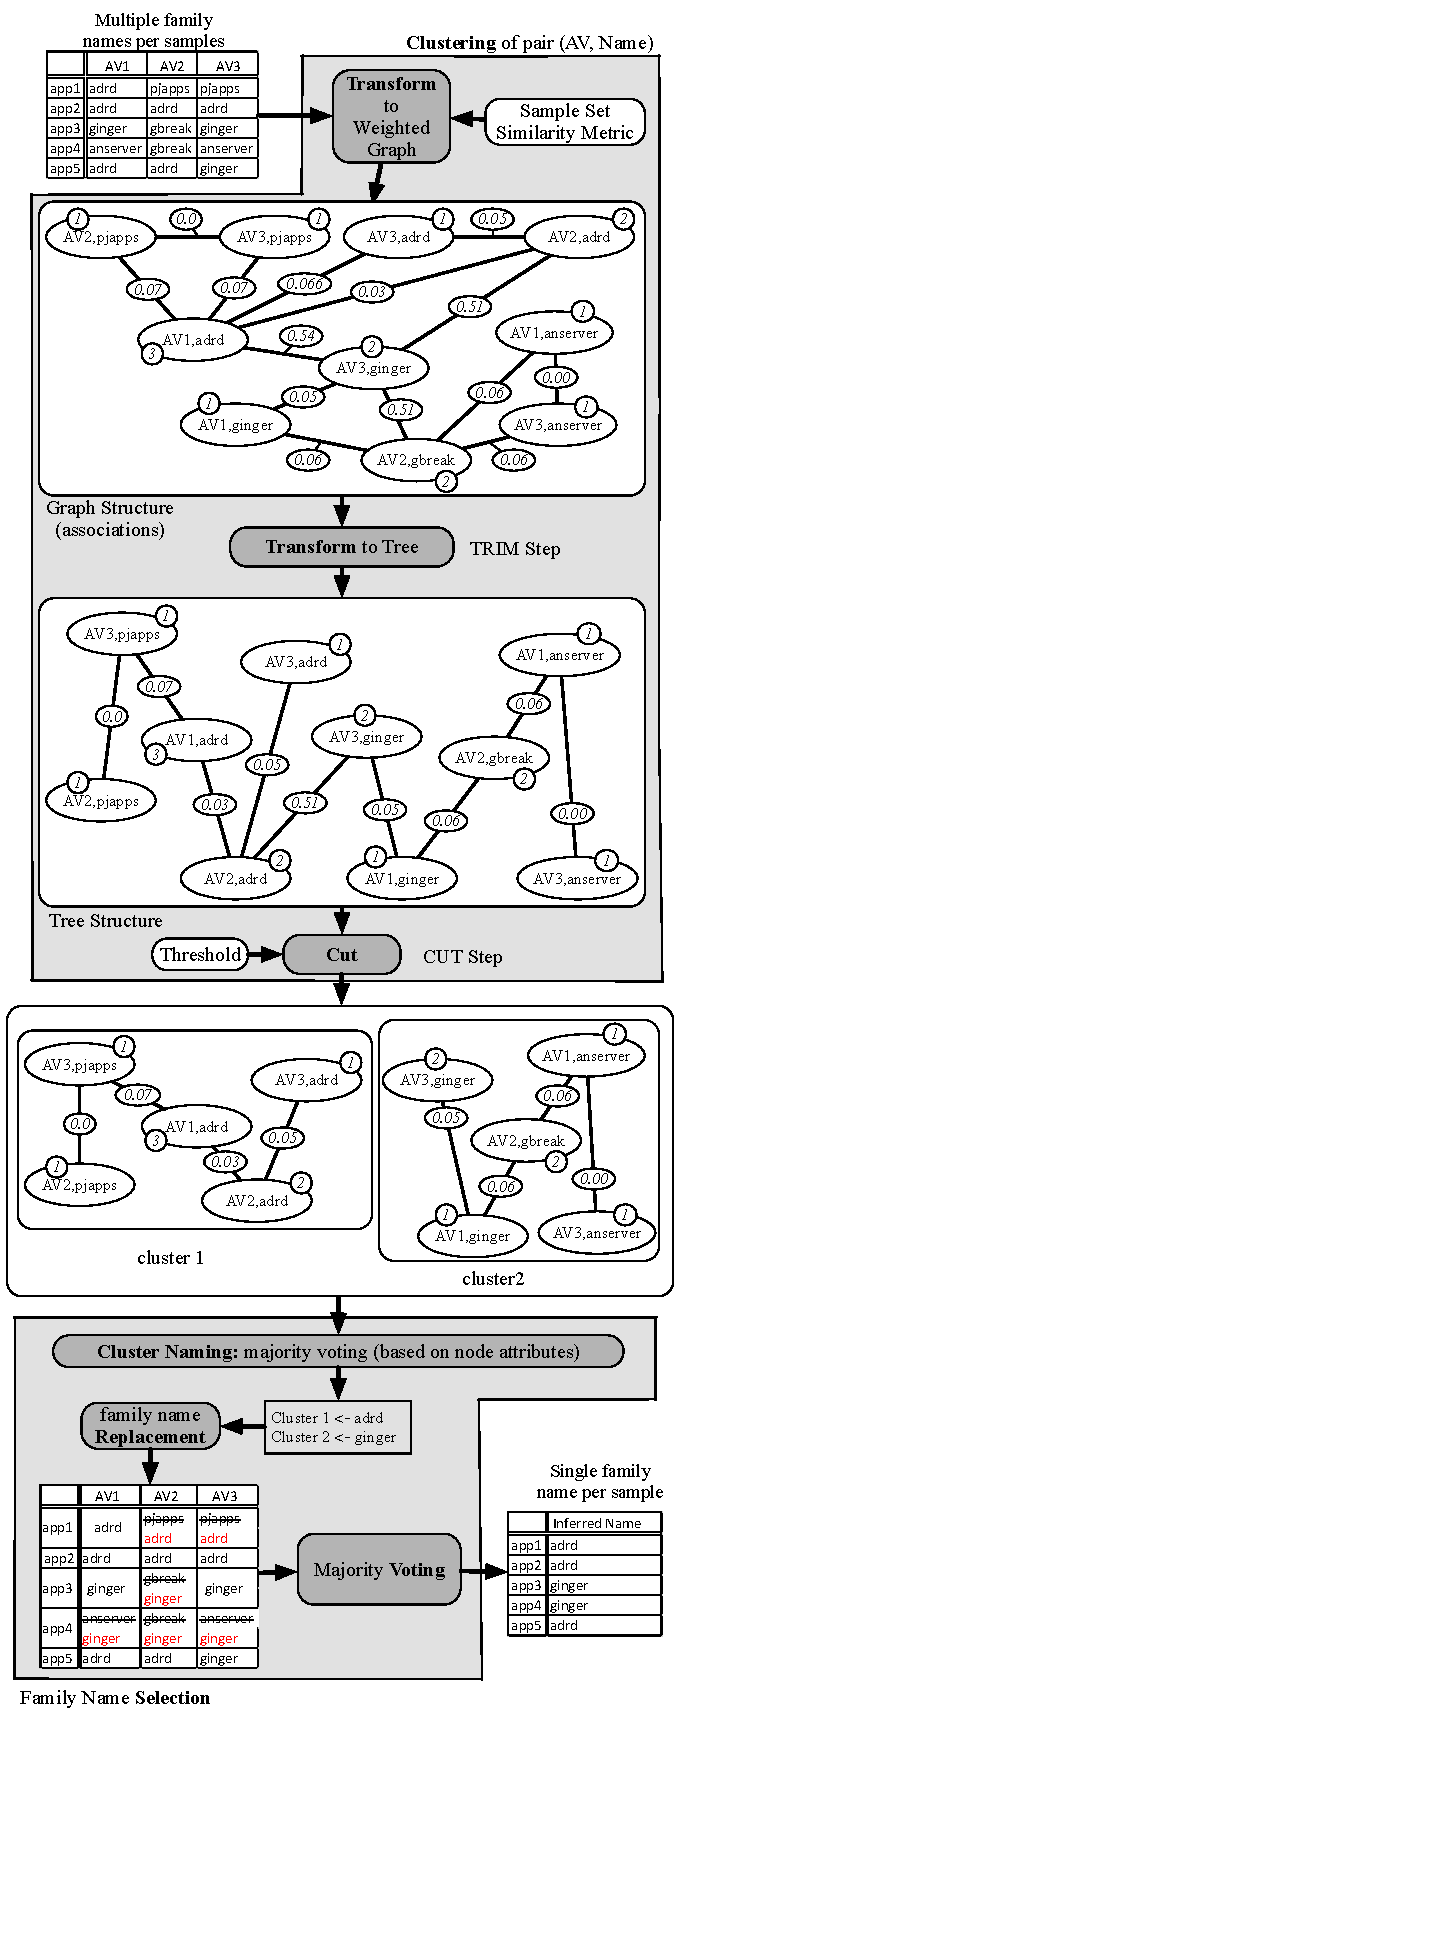
\includegraphics[height=\textheight]{figures/euphony/clustering03.pdf}
	\caption{Second stage - clustering \& Third stage - inference of family name}
	\label{figure:euphony:clustering}
\end{figure}

After parsing malware labels to identify family names given by different antivirus to each sample, EUPHONY builds a graph representing the association links between family names based on their assignment on some samples.
Then, based on a threshold parameter that determines the granularity of grouping, clusters of family names are separated.
Figure~\ref{figure:euphony:clustering} provides an overview of the process.
In the rest of the chapter, we will often use the terms ``name'' instead of the full expression ``family name''.
\subsection{Associating family names}
At the end of the previous stage, EUPHONY has a new dataset where each sample is associated with multiple malware family names reported by antivirus.
These potentially syntactically different names may include mislabeling noises and misclassification errors, which make the process of selecting unique names more difficult.

We study the associations between antivirus family names to group together commonly related names.
We found that the most natural method to analyze potential associations was to construct a weighted graph $G = (N, E)$, where a node $n \in N$ represents a name that an antivirus assigned: $n = (av_a, name)$, and an edge $e = [(av_a, name_x), (av_b, name_y)] \in E$ indicates that both antivirus $av_a$ and $av_b$ have labeled the same sample with $name_x$ and $name_y$ respectively.
From the information attached to a node, EUPHONY can identify the corresponding Sample Set $S_{av_a,name}$ and computes, for each node, the size of its sample set (i.e., the number of times the family name is given by that antivirus in the dataset).
It also computes, for each edge, the overlapping between the related sample sets (i.e., the number of times antivirus agree on the name given at that node).
Both pieces of information are then used to compute the {\em Imbalance} and {\em Exclusion} metric, and eventually the {\em Sample Set Distance} metric, also taking into account the string distance between family names.
Imbalance and Exclusion metric values are used as edge attributes in the graph, while the Sample Set Distance metric value is used as the edge weight (in Figure~\ref{figure:euphony:clustering} only the edge weight is represented).
Note that the weight of an edge represents the degree to which the sample sets associated with the connected nodes are dissimilar: the lower the weight, the more likely both sample sets belong to the same cluster.
\subsection{Clustering family names}
Given the large number of associations that we have observed among family names in our datasets, we expect the weighted graph to be highly connected and thus include very few identifiable subgraphs.
For instance, a generic name can create additional edges with more specific names and thus tie together components that were otherwise weakly related.
Processing mistakes during label fields extraction can also introduce fake associations among family names.
It is therefore essential to remove such undesired associations from the graph and only keep subgraphs with strongly related nodes.
To that end, we build a technique that comprises two successive steps, referred to as TRIM and CUT:

\begin{itemize}
	\item In the TRIM step, we use Prim's algorithm~\cite{prim_shortest_1957} to transform the graph into a Minimum Spanning Tree (i.e., the sum of its edge weights is minimum). The goal of this operation is to reduce the complexity of the original structure and keep the most similar edges as long as they do not introduce cycles in the graph. The complexity of this algorithm is $O(|E|\log |N|)$ in our current implementation.
	\item The CUT step takes the tree structure and applies a filter function to remove edges whose weights exceed a given threshold value. As a result, the input tree is divided into connected components that can be interpreted as clusters of strongly related family names. The complexity of this algorithm is $O(|E|)$ in our implementation.
\end{itemize}

\subsection{Inferring family names}
In the last stage, we study the relation between the different family names to assess the prevalence of predominant naming schemes used by the different antivirus.
In particular, we created a list of associations that put in relation all family names within the cluster where they are grouped.
More specifically, we first associate a single name to each cluster.
This name is inferred as the most frequent name present in the cluster by taking into account the attribute of each node.
In the step illustrated at the bottom of Figure~\ref{figure:euphony:clustering}, cluster 1 is associated with $adrd$ and cluster 2 to $ginger$.
Then, each family name present in a cluster is replaced by the cluster name.
For instance, in Figure~\ref{figure:euphony:clustering}, $pjapps$ given by $AV2$ is replaced by $adrd$.
More generally, in this example, all occurrences of $pjapps$ are replaced by $adrd$ and all occurrences of $anserver$ or $gbreak$ by $ginger$.

Once the replacements are done, to infer a single family name per sample, we implement a majority voting where we compute the frequency of each family name and select the most frequent one per sample.
In the case of a tie, we use the highest frequency of the names within the dataset to choose between the candidates and break the conflict.
\section{Analysis of EUPHONY results}
\subsection{Datasets and metrics}
The evaluation of EUPHONY is based on two different sets of samples: (i) \textit{reference datasets}, and (ii) an \textit{in the wild dataset}.
We next describe the source of each of the datasets used (see Table~\ref{table:euphony:datasets} for a summary) and the metrics used to evaluate our approach.

\textbf{Reference datasets:} These datasets have been distributed by the research community together with a reference ground truth of malware families, and have been widely used in the literature recently~\cite{arp_drebin:_2014, dash_droidscribe:_2016,lindorfer_marvin:_2015}.
For our study, we consider {\em MalGenome}~\cite{zhou_dissecting_2012}, a dataset manually vetted and collected between 2008 and 2010, and which includes 1\,262 samples regrouped into 44 families.
Similarly to previous works~\cite{monrose_avclass:_2016}, we update this dataset by grouping into a single family all variants of $DroidKungFu$ ($DroidKungFu1$, $DroidKungFu2$, $DroidKungFusApp$, etc.).
Additionally, we also consider {\em Drebin}~\cite{arp_drebin:_2014}, a dataset collected between 2010 and 2012, and which includes all samples from {\em MalGenome} as well as an additional set of 3\,998 more samples.
{\em Drebin} includes 178 families.

\textbf{In the wild dataset:} We collected recent samples from {\em Androzoo}~\cite{allix_androzoo:_2016}, a repository that shares samples from a variety of sources as well as their antivirus labels provided by {\em VirusTotal}.
For our study, we leveraged the public download API and retrieved 402\,600 samples created between January 2015 and August 2016\footnote{{\em Androzoo} bases its timeline on the DEX compilation date.}.
We ensured that all samples were classified as malware by at least one antivirus\footnote{Overall, the samples were labeled by 63 antivirus}.

\begin{table}[!ht]
    \centering
    \caption{Datasets used in EUPHONY evaluation}
    \resizebox{0.9\linewidth}{!}{
        \begin{tabular}{|r|c|r|c|c|r|}
            \hline
            \textbf{Reference}                        & \textbf{Wild}   & \textbf{Samples} & \textbf{Families} & \textbf{Anti-Virus} & \textbf{Collection Period} \\
            \hline
            {\em MalGenome}~\cite{zhou_dissecting_2012}       & \ding{55} & 1\,262   &       44 &        58 & 08/2008 - 10-2010 \\
            {\em Drebin}~\cite{arp_drebin:_2014}             & \ding{55} & 5\,260   &      178 &        57 & 08/2010 - 10/2012 \\
            {\em Androzoo}~\cite{allix_androzoo:_2016}   & \ding{51} & 402\,600 &  unknown &        63 & 01/2015 - 08/2016 \\
            \hline
        \end{tabular}
    }
    \label{table:euphony:datasets}
\end{table}


\textbf{Evaluation metrics:} Let $S$ be a sample dataset, $G = \{G_1, \dots, G_s\}$ be the set of $s$ ``ground truth'' clusters from $S$, and $C = \{C_1, \dots, C_n\}$ be the set of $n$ clusters output by a given tool over $S$.
Similarly to previous works~\cite{monrose_avclass:_2016}, we define the following metrics:

\begin{itemize}
	\item \textbf{Precision:} $Prec = \frac{1}{n} \times \sum^n_{j=1} \max_{k=1,\dots,s}(|C_j \cap G_k|)$
	\item \textbf{Recall:} $Rec = \frac{1}{s} \cdot \sum^s_{k=1} \max_{j=1,\dots,n}(|C_j \cap G_k|)$
	\item \textbf{F1 score:} $F1 = 2 \times \frac{Prec \times Rec}{Prec + Rec}$
\end{itemize}

While precision measures the effectiveness of a tool to map outputted clusters into ground truth clusters, recall quantifies the effectiveness of the tool to map ground truth clusters into outputted clusters.
Finally, the F Measure represents the harmonic mean between precision and recall.

In this chapter, we first investigate the precision and recall reported when clustering malware samples in the reference datasets.
These metrics allow us to compare our approach with previous works quantitatively~\cite{monrose_avclass:_2016}.
We then use the samples collected in the wild to evaluate several statistical metrics such as the number of families, the number of singletons and the most relevant labels.
\subsection{Performance evaluation}

\begin{figure}[!ht]
	\centering
	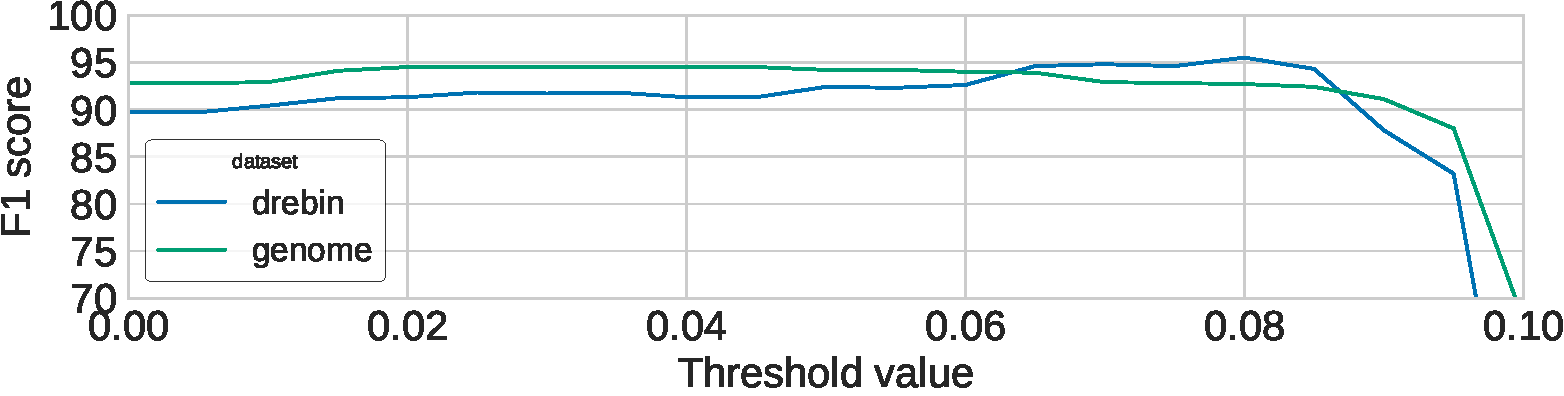
\includegraphics[width=\linewidth]{figures/euphony/threshold.pdf}
	\caption{Parameter selection of the threshold value}
	\label{figure:euphony:threshold}
\end{figure}

EUPHONY uses a threshold to control the clustering sensitivity by breaking edges whose weight exceeds the given value.
On Figure~\ref{figure:euphony:threshold}, we observed that a threshold of $0.07$ represented an excellent trade-off between noise reduction and accuracy.

We now evaluate the performance reported over the reference datasets.
The leftmost part of Table~\ref{table:euphony:labelled} shows the precision, recall and F1 measure for EUPHONY.
Results show that clustering {\em MalGenome} is, overall, more challenging than clustering {\em Drebin}, with a F1 measure of 92.7\% and 95.5\% respectively.

These results can be explained by looking at the precision, which shows that not all predicted clusters can be mapped to their respective reference clusters.
Interestingly, the score obtained for the recall indicates that almost all referenced clusters (i.e., 99.7\% of the malware families) in {\em MalGenome} have been correctly predicted.
Instead, only 96.1\% of the referenced clusters in {\em Drebin} have been correctly predicted.

\begin{table*}
    \centering
    \caption[Performance of EUPHONY against state-of-the-art]{Performance of EUPHONY against state-of-the-art (in \%)}
    \label{tab:avclass-full}
    \resizebox{\textwidth}{!}{
        \begin{tabular}{|c|cccc|ccc|ccc|ccc|ccc|}
                    \hline
                    & \multicolumn{4}{c|}{\textbf{EUPHONY}} & \multicolumn{12}{c|}{{\em \textbf{AVClass}}} \\
                    \hline
                    & \multicolumn{4}{c|}{-} & \multicolumn{3}{c|}{\textbf{{\em AVClass} Config 1}} & \multicolumn{3}{c|}{\textbf{{\em AVClass} Config 2}} & \multicolumn{3}{c|}{\textbf{{\em AVClass} Config 3}} & \multicolumn{3}{c|}{\textbf{{\em AVClass} Config 4}} \\
                    & \multicolumn{4}{c|}{- } & \multicolumn{3}{c|}{\em as reported in~\cite{monrose_avclass:_2016}} & \multicolumn{3}{c|}{\em with default files in Git} & \multicolumn{3}{c|}{\em new aliases only} & \multicolumn{3}{c|}{\em new generics \& aliases} \\
            \hline
            Dataset       & Prec  & Rec  & F1   & \#  &     Prec & Rec  & F1   &    Prec & Rec  & F1   &     Prec & Rec  & F1   & Prec & Rec  & F1   \\
            \hline
            {\em MalGen.} &  86.7 & 99.7 & 92.7 & 33  &     87.2 & 98.8 & 92.6 &    86.5 & 98.0 & 91.9 &     86.2 & 99.0 & 92.1 & 53.9 & 65.2 & 59.0      \\
            {\em Drebin}  &  95.0 & 96.1 & 95.5 & 142 &     95.2 & 92.5 & 93.9 &    95.4 & 93.0 & 94.2 &     95.6 & 90.6 & 93.0 & 29.6 & 69.8 & 41.6        \\
            \hline
        \end{tabular}
    }
    \label{table:euphony:labelled}
\end{table*}


When analyzing {\em MalGenome} results, we observe that some antivirus prefer to combine some reference clusters to form one single super family.
For instance, families $ADRD$ (22 samples) and $Pjapps$ (58 samples), are perceived as one large family called $Pjapps^*$ (with 80 samples).
Similarly, $BaseBridge$ (122 samples) and $AnserverBot$ (187 samples) are perceived as $Basebridge^*$ (with 309 samples).
This is understandable as authors in~\cite{zhou_dissecting_2012} believe that $AnserverBot$ evolved from $BaseBridge$, inheriting common features.
Other recent works have also confirmed this and pointed out that some other families are also strongly related to each other~\cite{suarez-tangil_dendroid:_2014}.
Based on this, one can conclude that the perception of the antivirus is, in some general cases, more coarse-grained.
Thus, they can treat two similar clusters as one single family.

As for the results obtained with {\em Drebin}, we found some cases where the antivirus agree on using a more fine-grained definition of some families than the one given in the reference ground truth.
For example, most of the samples from the reference family $Opfake$ (952 samples) are subdivided into two sub families, i.e., $Opfake$ (546 samples) and $SMSSend$ (25 samples).
Similarly, most of the samples in $ExploitLinuxLotoor$ (70 samples) are subdivided into three subfamilies: $Lotoor^*$ (58 samples), $GingerBreak$ (9 samples) and $AsRoot$ (8 samples).
\subsubsection*{Comparison against the state-of-the-art}
To provide further insights on the performance achieved by EUPHONY, we compare our results with {\em AVClass}~\cite{monrose_avclass:_2016}.
Since the authors have analyzed their approach on {\em MalGenome} and {\em Drebin} datasets, we use the results in their paper as our evaluation baseline (Table~\ref{table:euphony:labelled}, {\em AVClass} Config 1).
We also replicate their experiments by taking into account the difference between the inputs requirements of both tools.
On the one hand, EUPHONY uses a small list of some well-known words (\underline{not including family names}) about malware labels.
On the other hand, {\em AVClass } requires a list of malware families to construct a set of \textit{generics tokens} and \textit{aliases}.
These sets are built in a two-step process.
First, {\em AVClass } uses the list of malware families to distinguish these family tokens from other so-called \textit{generics tokens} (e.g.,
types, platforms, information).
Second, {\em AVClass} strips generics tokens from malware labels to discover \textit{aliases} among malware family names.
Finally, the sets of \textit{generics tokens} and \textit{aliases} are leveraged to produce the final output of the tool: a single family name per malware sample using a plurality voting.
Several factors may thus impact the performance of AVClass, including the exhaustiveness of the inputted list of malware families, and the error rate in the generation of the sets of generics and aliases.
Consequently, we consider three different scenarios for our evaluation:

\begin{itemize}
	\item An updated version of {\em AVClass}---we use the last version of the tool released on GitHub, taking into account recent code fixes, as well as updates to complete the list of generic terms and aliases\footnote{AVClass repository cloned on Oct 24, 2016. Commit head: 80c14adcc29978ab813b41c73dd485072e576140}. The results are reported in Table~\ref{table:euphony:labelled}, {\em AVClass} Config 2.
	\item Automatic inference of \textit{aliases} only---we use the authors' script with the default settings to generate a list of aliases based on our two reference datasets (Table~\ref{table:euphony:labelled} Config 3).
	\item Automatic inference of both \textit{generics} and \textit{aliases}---we use the authors' scripts with the default settings on the union of our two reference datasets to build the knowledge necessary to {\em AVClass}'s functioning (Table~\ref{table:euphony:labelled} Config 4).
\end{itemize}

All results are reported in Table~\ref{table:euphony:labelled}.
For all four configurations, EUPHONY performs better than {\em AVClass} in terms of F1 score (harmonic mean between precision and recall).
Nonetheless, we observed that their precision is comparable to ours in those configurations where prior knowledge (aliases and generic terms) is provided.
When we inferred both (i) aliases, and (ii) aliases and generic terms using the samples given in the reference datasets (i.e.,: {\em MalGenome} and {\em Drebin})\footnote{Note that {\em AVClass} published results~~\cite{monrose_avclass:_2016} were obtained using the knowledge on aliases and generics that was built from larger datasets}, we observed that the performance drops drastically.
Typical families included in Config.
4 are: android (537 samples), trojan (377 samples) and basebridge (68 samples).
These observations show that the performance of {\em AVClass} is driven by the input of an initial knowledge---which should be collected by the final user.
In contrast, EUPHONY does not require any guiding process or pre-defined knowledge of the families.
The only prior knowledge required by our framework is a basic understanding of some common types of malware (i.e., trojan, virus, etc.), execution platforms (i.e., android, linux, Win32, etc.) and information (e.g., dll, pak, gen).
\subsection{Evaluation of samples in the wild}
This section reports our experiments in the wild.
We analyze the number of samples that EUPHONY can group with respect to {\em AVClass}.
Note that in this section we report results using the same experimental setting used above.
As for {\em AVClass}, we choose the most favorable configuration\footnote{This is, using the default lists of aliases and generics collected by the authors.
	These lists may have been manually improved to guarantee the labeling system out of the lab}.
Table~\ref{table:euphony:androzoo} summarizes the results obtained on the {\em Androzoo} dataset.

\begin{table}[!ht]
    \centering
    \caption[Results of EUPHONY for {\em Androzoo}]{Results of EUPHONY for {\em Androzoo} (402\,600 samples)}
    \resizebox{0.6\linewidth}{!}{
        \begin{tabular}{|c|c|c|c|c|}
            \hline
                            & \textbf{Labeled}  & \textbf{Clusters} & \textbf{Singletons} & \textbf{Runtime} \\
            \hline
            EUPHONY       & 319\,100 & 735      & 165        & 216s \\
            {\em AVClass} & 178\,471 & 453      & 135        & 114s \\
            \hline
        \end{tabular}
    }
    \label{table:euphony:androzoo}
\end{table}


Results show that EUPHONY managed to cluster 79\% of the samples (319\,100 out of 402\,600).
In contrast, {\em AVClass} clustered 44\% (178\,471 out of 402\,600).
These results mean that a practitioner using {\em AVClass} would not obtain labels for more than half of the recent dataset.
This can be partly explained by the strategy used by {\em AVClass} to handle generic terms in labels, as well as aliases in family names.

On the contrary, our approach does not present distinctions between generic and specific malware families, and may thus find more associations.
This can further provide a better understanding of the appropriate set of samples in every cluster.
In this regard, EUPHONY has split the dataset into 735 clusters and produces 165 clusters with one single sample (namely, singletons).
Instead, {\em AVClass} proposed 453 clusters and 135 singletons.
Note that the runtime overhead of EUPHONY is negligible compared to {\em AVClass}, even in this setting where the creation of \textit{generics tokens} and \textit{aliases} for {\em AVClass} was skipped.

\begin{table}
    \centering
    \caption{Top 10 clusters of EUPHONY and {\em AVClass}}
    \label{table:euphony:unlabelled}
    \resizebox{0.5\linewidth}{!}{
        \begin{tabular}{|c|r||c|r|}
            \hline
            \multicolumn{2}{|c||}{\textbf{EUPHONY}} &\multicolumn{2}{|c|}{\textbf{AVClass}} \\
            \hline
            \textbf{Family}   & \textbf{Samples} & \textbf{Family}   & \textbf{Samples}\\
            \hline
            dowgin    & 37\,739 & kuguo    & 38\,532\\
            kuguo     & 25\,005 & dowgin   & 22\,643\\
            addisplay & 20\,862 & secapk   & 20\,492\\
            jiagu     & 20\,705 & airpush  & 13\,209\\
            anydown   & 19\,621 & jiagu    & 8\,987\\
            secapk    & 18\,224 & smsreg   & 8\,427\\
            generic   & 17\,836 & feiwo    & 7\,399\\
            agent     & 17\,596 & revmob   & 6\,376\\
            inmobi    & 16\,203 & leadbolt & 5\,348\\
            airpush   & 13\,267 & anydown  & 5\,147\\
            \hline
        \end{tabular}
    }
\end{table}


Table~\ref{table:euphony:unlabelled} shows the Top 10 clusters (in terms of size) for both EUPHONY and {\em AVClass}.
Both approaches report clusters of the same order of magnitude and with similar family names.
This table indicates that EUPHONY reaches similar conclusions than {\em AVClass} for the most popular families, but without prior knowledge of generic families.

We can also observe that our approach can deal with generic antivirus labels.
For instance, a common field used by antivirus is ``trojan.androidos.generic.a'', with 94\,255 occurrences (4\%).
We can further observe 576\,261 occurrences (23\%) of the string ``gen'' in the list of labels.
This result contrast with the most occurring family, $Dowgin$, with 311\,593 times (14\%).
Moreover, it explains the lack of coverage reported by {\em AVClass}.
We position here that being aware of these types of clusters are important to filter out samples that might interfere with the proper classification of other clusters.
In practice, adware and other type of grayware~\cite{suarez-tangil_evolution_2014} could be identified.
Nevertheless, to account for corner cases where a generic term is selected as a family name, practitioners can inject into EUPHONY their knowledge on how a specific token must be associated with a label field.
Since a significant portion of samples remained unlabeled by {\em AVClass} and EUPHONY, we only consider the subset of samples that are labeled by both tools to investigate the similarities and differences among reported clusters.
We provide in Table~\ref{table:euphony:top10} the statistics on the new Top 10 clusters (dropping samples that are unlabeled by either tool) and information on the extent to which they overlap.
Most top families strongly overlap.
For example, $Dogwin$, the most prevalent family in EUPHONY, overlaps with the also labeled $Dogwin$ family in {\em AVClass} with a ratio of 95\%.
For 7 of the top 10 clusters given by EUPHONY, we find that the corresponding cluster by {\em AVClass} overlaps at over 85\%.
If we take the particular case of samples labeled as $Kuguo$ by {\em AVClass}, EUPHONY splits them into mainly three families ($kuguo$, $addisplay$, $hiddeninstall$) with an overlap of 99\%, 54\%, and 93\% respectively.

\begin{table}[!ht]
    \centering
    \caption{Top 10 clusters of EUPHONY compared to {\em AVClass}}
    \label{table:euphony:top10}
    \resizebox{0.7\linewidth}{!}{
        \begin{tabular}{|cr|cr|rr|}
            \hline
            \multicolumn{2}{|c|}{\textbf{EUPHONY}} & \multicolumn{2}{c|}{\textbf{{\em AVClass}}} & \multicolumn{2}{c|}{\textbf{Intersection}} \\
            \hline
            \textbf{Family}    & \textbf{samples} & \textbf{Family}  & \textbf{samples} & \textbf{samples} & \textbf{overlap (in \%)} \\
            \hline
            dowgin    & 33\,297   & dowgin  & 22\,617   & 21\,035   & 93.0 \\
            kuguo     & 24\,273   & kuguo   & 38\,532   & 24\,072   & 99.2 \\
            secapk    & 17\,889   & secapk  & 20\,492   & 17\,825   & 99.6 \\
            addisplay & 11\,203   & kuguo   & 38\,532   & 6\,055    & 54.0 \\
            airpush   & 10\,055   & airpush & 13\,202   & 10\,017   & 99.6 \\
            jiagu     & 7\,215    & jiagu   & 8\,987    & 7\,211    & 99.9 \\
            smsreg    & 6\,294    & smsreg  & 8\,427    & 5\,819    & 92.5 \\
            agent     & 6\,088    & feiwo   & 7\,399    & 1\,014    & 16.7 \\
            revmob    & 6\,061    & revmob  & 6\,376    & 6\,058    & 99.9 \\
            generic   & 5\,663    & anydown & 5\,147    & 1\,890    & 36.7 \\
            \hline
        \end{tabular}
    }
\end{table}


\section{Support of threat intelligence services}
As the lack of human experts disrupts our ability to analyze malware in the large~\cite{ics2_cybersecurity_2018}, threat intelligence services will become essential to enable the detection and the classification of Android malware further.
Online services such as {\em VirusTotal} already contribute to this effort by providing diversified antivirus labels for malware samples.
However, the results of {\em VirusTotal} cannot be leveraged as-if to support the creation of ground truth datasets due to the lack of naming convention between antivirus engines.
With EUPHONY, we developed a state-of-the-art approach that unifies the output of antivirus systems and assigns valuable information from the knowledge embedded in antivirus labels.

EUPHONY improves over {\em AVClass} by overcoming its main limitations of requiring a substantial amount of initial knowledge on malware families and antivirus vendors to bootstrap the labeling process.
Moreover, reference datasets need to be regularly updated without prior knowledge on generic terms that antivirus vendors use to label samples as new malware families appear.
From a small and relatively stable list of common tokens, EUPHONY can (1) infer missing information on tokens in antivirus label strings using heuristics, and (2) group similar families together according to a comprehensive distance metric that takes into account typos in naming, imbalance in label assignment among antivirus sample sets, and overlapping of sets.
While EUPHONY can be used off-the-shelf, without any requirement of expertise on malware labels, advanced users may also build on top of our framework and specify their heuristics, metrics or knowledge of malware labels to build their unification process.

Since the creation of better ground truth datasets is an important objective toward the development and the adoption of machine learning based systems, the security community must continue to provide a better interpretation on the relation between malware families and their structural features.
Recent approaches~\cite{suarez-tangil_droidsieve:_2017} have been efficient at identifying syntactic and resource-centric features that characterize Android malware.
We position that adding these features to our algorithm could contribute to alleviate disagreements among antivirus vendors and support the extraction of malicious artifacts associated with specific malware families.
